\documentclass{article}
\usepackage{fancyhdr}
\usepackage{titlesec}
\usepackage{graphicx}
\graphicspath{ {./img/} }

\pagestyle{fancy}
\fancyhf{}
\lhead{Modul 3 Praktikum Jaringan Komputer}
\rfoot{\footnotesize Page \thepage}
\lfoot{\footnotesize Mahyus Ihsan, S.Si, M.Si \newline Jurusan Informatika Universitas Syiah Kuala \newline Modul oleh : Diky Wahyudi, Furqan Al Ghifari, Rendika Rahmaturrizki}
\renewcommand{\headrulewidth}{1pt}
\renewcommand{\footrulewidth}{1pt}

\titleformat*{\section}{\small\bfseries}

\begin{document}
    \begin{center}
        \textbf{Modul 3 Praktikum Jaringan Komputer}

        \textbf{Address Resolution Protocol (ARP)}
    \end{center}

    \section*{Deskripsi Singkat}
    ARP adlah sebuah protokol dalam TCP/IP Protocol Suite yang bertanggungjawab dalam melakukan resolusi alamat IP ke dalam alamat Media Access Control. 
    Dalam sebuah \textbf{Ethernet Frame Fields} terdapat MAC address dari si pengirim/\textit{Sources} dan si penerima/\textit{Destination}.Pada awalnya si pengirim tidak mengetahui MAC address si penerima, sehingga dibutuhkan ARP untuk mendapatkan MAC address dari si penerima.

    \section*{Tujuan}
    \begin{enumerate}
        \item Dapat mengetahui fungsi ARP
        \item Dapat memahami cara kerja ARP
    \end{enumerate}

    \begin{flushleft}
        \textbf{Materi 1 - Address Resolution Protocol (ARP)}
        \newline

        Setiap perangkat memiliki MAC address yang unik dan berbeda dari yang lain. Ketika perangkat akan mengirimkan sebuah paket maka diperlukan MAC address si penerima, maka untuk mendapatkan MAC address tersebut diperlukan ARP.
        \begin{description}
            \item[Source MAC Address] adalah MAC address si pengirim.
            \item[Destination MAC address] adalah MAC address si penerima, jika penerima bedara di dalam jaringan yang sama maka MAC addres tertuju pada perangkat tujuan.
            Sedangkan jika penerima berada di jaringan lain, maka MAC address tujuan akan tertuju pada default gateway.
        \end{description}

        Untuk melakukan simulasi bagaimana cara ARP bekerja bisa menggunakan packet tracer
        \begin{enumerate}
            \item Silahkan buka \textbf{9.2.9-packet-tracer---examine-the-arp-table.pkg} yang ada pada CiscoPacket.zip
            \item Klik dua kali pada komputer dengan IP \textbf{172.16.31.2} kemudian buka aplikasi \textbf{Command Prompt} kemudian ketik \textbf{arp -d} pada command prompt untuk membersihkan cache arp pada komputer.
            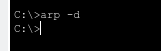
\includegraphics[scale=1.5]{1-arp-d.png}

            \item Kemudian masuk kedalam mode simulasi. Klik \textbf{Show All/None} kemudian pilih \textbf{ARP dan ICMP saja}
            
            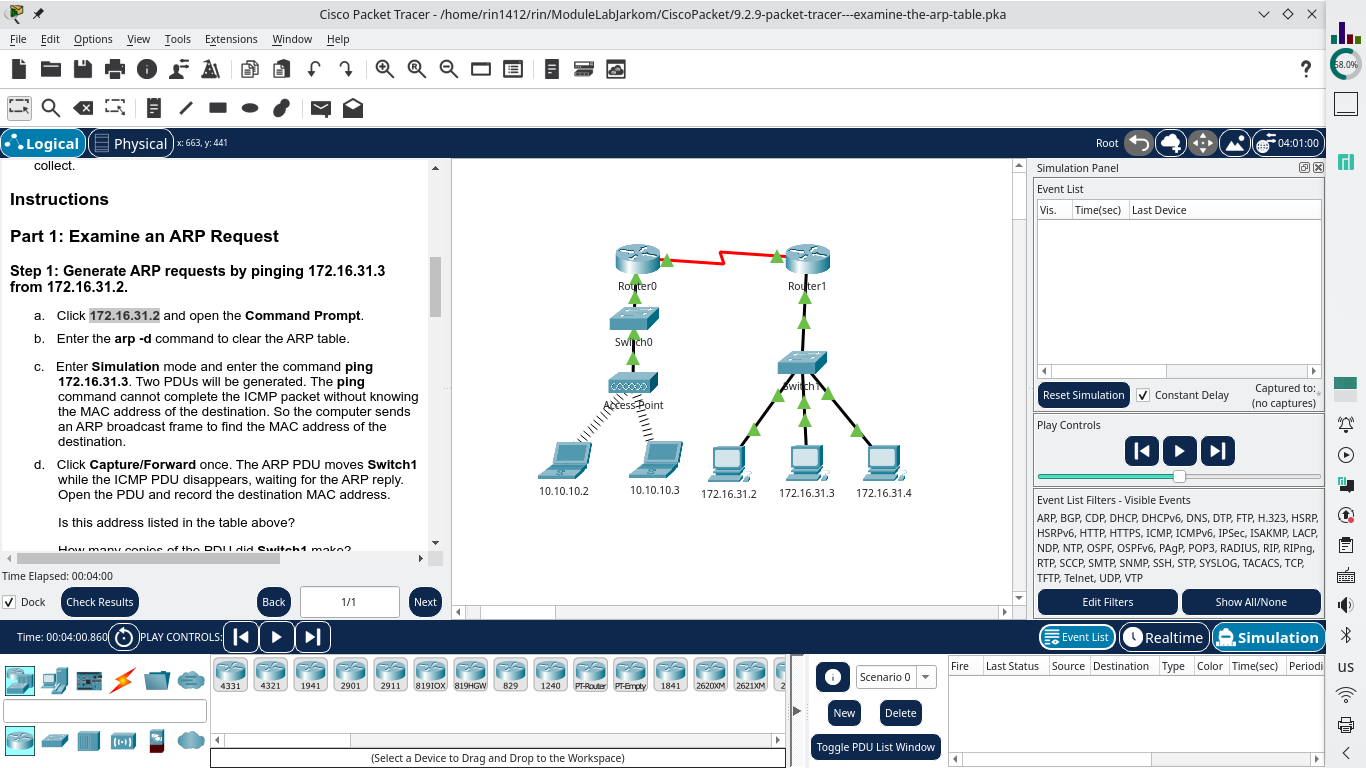
\includegraphics[scale=0.3]{1-sim.png}
            
            \item Kemudian lakukan ping dari komputer dengan IP \textbf{172.16.31.2} ke komputer dengan IP \textbf{172.16.31.3}
            
            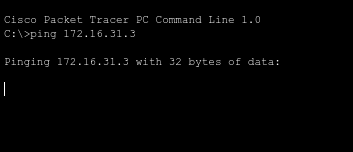
\includegraphics[scale=0.6]{1-ping.png}
            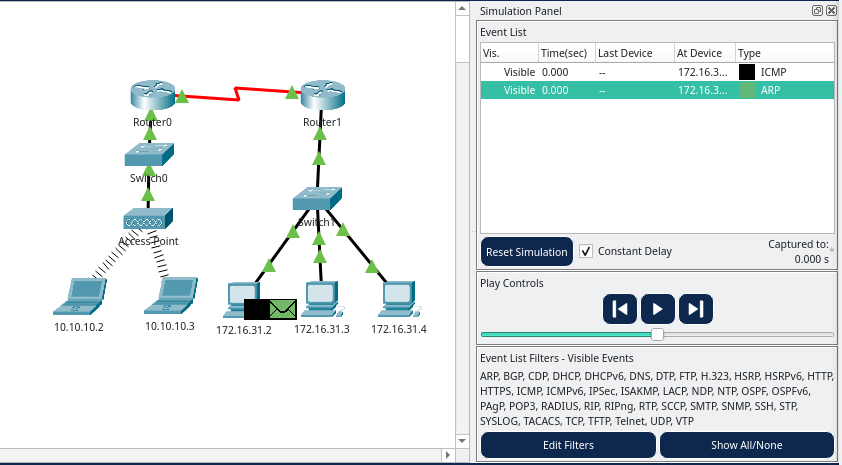
\includegraphics[scale=0.5]{1-arp-sim.png}

            \item Dalam menu \textbf{Play Control} silakan klik tombol \textit{play} untuk melanjutkan proses pada simulasi.
            Apa yang terjadi pada table event list ?
            Apa saja yang terjadi pada komputer si pengirim dan si penerima ?
            Bagamana cara kerja ARP ?

            \item Setelah melakukan ping, cek \textbf{ARP table} dengan perintah \textbf{arp -a} pada \textbf{Command Prompt}. Disana terdapat IP dan MAC address dari komputer si penerima.
            
            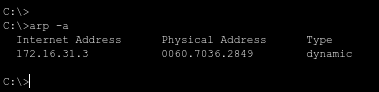
\includegraphics{1-arp-a.png}

            \item Lakukan ping sekali lagi dari komputer dengan IP \textbf{172.16.31.2} ke komputer dengan IP \textbf{172.16.31.3}. Apa yang terjadi ? Apakah komputer menjalankan protokol ARP lagi ?
        \end{enumerate}
    \end{flushleft}
\end{document}
